\documentclass{standalone}
\usepackage{tikz}
\usepackage{bm}
\usetikzlibrary{shapes,arrows,positioning,decorations.markings}

\begin{document}
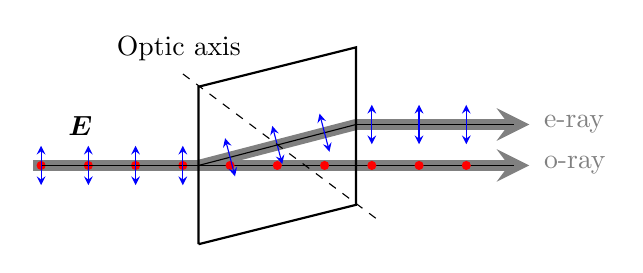
\begin{tikzpicture}
    
    \node at (-1.5, 1.5) {$\bm{E}$};
    
    % E-field
    \draw[->, gray, line width=4, >=stealth] (-2.1,1)--(4.2,1) node[right] {o-ray};
    \draw[gray, line width=4] (0,1)--(2,1.52) node[below] {};
    \draw[->, gray, line width=4, >=stealth] (2,1.52)--(4.2,1.52) node[right] {e-ray};
    
    % Perp. field component
    \draw [postaction={decorate,decoration={markings, mark=between positions 0 and 3 step 0.1 with {\draw [thin,red,fill=red] circle (0.05);}}}](-2,1) -- (4,1);
    
    % Parallel component.
    \draw [postaction={decorate,decoration={markings, mark=between positions 0 and 3 step 0.3 with {\draw [<->,blue,thin, >=stealth] (0,-0.25) -- (0,0.25);}}}](-2,1) -- (0,1);
    
    \draw [postaction={decorate,decoration={markings, mark=between positions 0.2 and 3 step 0.3 with {\draw [<->,blue,thin, >=stealth] (0,-0.25) -- (0,0.25);}}}](0,1)--(2,1.52);
    
    \draw [postaction={decorate,decoration={markings, mark=between positions 0.1 and 2.1 step 0.3 with {\draw [<->,blue,thin, >=stealth] (0,-0.25) -- (0,0.25);}}}](2,1.52)--(4,1.52);
    
    % Calcite square thing
    \draw[thick] (0,0)--(0,2)--(2,2.5)--(2,0.5)--(0,0);
    
    % O-axis
    \draw[dashed] (2.25,0.33)--(-0.25,2.2) node[above] {Optic axis};

    
\end{tikzpicture}
\end{document}